%% bare_conf.tex
%% V1.4b
%% 2015/08/26
%% by Michael Shell
%% See:
%% http://www.michaelshell.org/
%% for current contact information.
%%
%% This is a skeleton file demonstrating the use of IEEEtran.cls
%% (requires IEEEtran.cls version 1.8b or later) with an IEEE
%% conference paper.
%%
%% Support sites:
%% http://www.michaelshell.org/tex/ieeetran/
%% http://www.ctan.org/pkg/ieeetran
%% and
%% http://www.ieee.org/

%%*************************************************************************
%% Legal Notice:
%% This code is offered as-is without any warranty either expressed or
%% implied; without even the implied warranty of MERCHANTABILITY or
%% FITNESS FOR A PARTICULAR PURPOSE! 
%% User assumes all risk.
%% In no event shall the IEEE or any contributor to this code be liable for
%% any damages or losses, including, but not limited to, incidental,
%% consequential, or any other damages, resulting from the use or misuse
%% of any information contained here.
%%
%% All comments are the opinions of their respective authors and are not
%% necessarily endorsed by the IEEE.
%%
%% This work is distributed under the LaTeX Project Public License (LPPL)
%% ( http://www.latex-project.org/ ) version 1.3, and may be freely used,
%% distributed and modified. A copy of the LPPL, version 1.3, is included
%% in the base LaTeX documentation of all distributions of LaTeX released
%% 2003/12/01 or later.
%% Retain all contribution notices and credits.
%% ** Modified files should be clearly indicated as such, including  **
%% ** renaming them and changing author support contact information. **
%%*************************************************************************


% *** Authors should verify (and, if needed, correct) their LaTeX
% *** system *** with the testflow diagnostic prior to trusting their
% *** LaTeX platform *** with production work. The IEEE's font choices
% *** and paper sizes can *** trigger bugs that do not appear when
% *** using other class files.  *** *** % The testflow support page is
% *** at: % http://www.michaelshell.org/tex/testflow/



\documentclass[conference]{IEEEtran}
% Some Computer Society conferences also require the compsoc mode option,
% but others use the standard conference format.
%
% If IEEEtran.cls has not been installed into the LaTeX system files,
% manually specify the path to it like:
% \documentclass[conference]{../sty/IEEEtran}





% Some very useful LaTeX packages include:
% (uncomment the ones you want to load)


% *** MISC UTILITY PACKAGES ***
%
%\usepackage{ifpdf}
% Heiko Oberdiek's ifpdf.sty is very useful if you need conditional
% compilation based on whether the output is pdf or dvi.
% usage:
% \ifpdf
%   % pdf code
% \else
%   % dvi code
% \fi
% The latest version of ifpdf.sty can be obtained from:
% http://www.ctan.org/pkg/ifpdf
% Also, note that IEEEtran.cls V1.7 and later provides a builtin
% \ifCLASSINFOpdf conditional that works the same way.
% When switching from latex to pdflatex and vice-versa, the compiler may
% have to be run twice to clear warning/error messages.






% *** CITATION PACKAGES ***
%
%\usepackage{cite}
% cite.sty was written by Donald Arseneau
% V1.6 and later of IEEEtran pre-defines the format of the cite.sty package
% \cite{} output to follow that of the IEEE. Loading the cite package will
% result in citation numbers being automatically sorted and properly
% "compressed/ranged". e.g., [1], [9], [2], [7], [5], [6] without using
% cite.sty will become [1], [2], [5]--[7], [9] using cite.sty. cite.sty's
% \cite will automatically add leading space, if needed. Use cite.sty's
% noadjust option (cite.sty V3.8 and later) if you want to turn this off
% such as if a citation ever needs to be enclosed in parenthesis.
% cite.sty is already installed on most LaTeX systems. Be sure and use
% version 5.0 (2009-03-20) and later if using hyperref.sty.
% The latest version can be obtained at:
% http://www.ctan.org/pkg/cite
% The documentation is contained in the cite.sty file itself.






% *** GRAPHICS RELATED PACKAGES ***
%
\ifCLASSINFOpdf
 \usepackage[pdftex]{graphicx}
  % declare the path(s) where your graphic files are
  % \graphicspath{{../pdf/}{../jpeg/}}
  % and their extensions so you won't have to specify these with
  % every instance of \includegraphics
  % \DeclareGraphicsExtensions{.pdf,.jpeg,.png}
\else
  % or other class option (dvipsone, dvipdf, if not using dvips). graphicx
  % will default to the driver specified in the system graphics.cfg if no
  % driver is specified.
  % \usepackage[dvips]{graphicx}
  % declare the path(s) where your graphic files are
  % \graphicspath{{../eps/}}
  % and their extensions so you won't have to specify these with
  % every instance of \includegraphics
  % \DeclareGraphicsExtensions{.eps}
\fi
% graphicx was written by David Carlisle and Sebastian Rahtz. It is
% required if you want graphics, photos, etc. graphicx.sty is already
% installed on most LaTeX systems. The latest version and documentation
% can be obtained at: 
% http://www.ctan.org/pkg/graphicx
% Another good source of documentation is "Using Imported Graphics in
% LaTeX2e" by Keith Reckdahl which can be found at:
% http://www.ctan.org/pkg/epslatex
%
% latex, and pdflatex in dvi mode, support graphics in encapsulated
% postscript (.eps) format. pdflatex in pdf mode supports graphics
% in .pdf, .jpeg, .png and .mps (metapost) formats. Users should ensure
% that all non-photo figures use a vector format (.eps, .pdf, .mps) and
% not a bitmapped formats (.jpeg, .png). The IEEE frowns on bitmapped formats
% which can result in "jaggedy"/blurry rendering of lines and letters as
% well as large increases in file sizes.
%
% You can find documentation about the pdfTeX application at:
% http://www.tug.org/applications/pdftex





% *** MATH PACKAGES ***
%
%\usepackage{amsmath}
% A popular package from the American Mathematical Society that provides
% many useful and powerful commands for dealing with mathematics.
%
% Note that the amsmath package sets \interdisplaylinepenalty to 10000
% thus preventing page breaks from occurring within multiline equations. Use:
%\interdisplaylinepenalty=2500
% after loading amsmath to restore such page breaks as IEEEtran.cls normally
% does. amsmath.sty is already installed on most LaTeX systems. The latest
% version and documentation can be obtained at:
% http://www.ctan.org/pkg/amsmath


\usepackage{fancyhdr}
\usepackage[caption=false,font=footnotesize]{subfig}

\renewcommand{\thispagestyle}[2]{}
\fancypagestyle{plain}{
	\fancyhead{}
	\fancyhead[C]{first page center header}
	\fancyfoot{}
	\fancyfoot[C]{first page center footer}
}
\pagestyle{fancy}

\headheight 20pt
\footskip 20pt

\rhead{}

%Enter the first page number of your paper below
\setcounter{page}{1}

\fancyhead[R]{\textit{(IJACSA) International Journal of Advanced
		Computer Science and Applications, \\ Vol. XXX, No. XXX, 2018}}
\renewcommand{\headrulewidth}{0pt}

%Footer
\fancyfoot[C]{www.ijacsa.thesai.org}
\renewcommand{\footrulewidth}{0.5pt}
\fancyfoot[R]{\thepage\ $|$ Page}


% *** SPECIALIZED LIST PACKAGES ***
%
%\usepackage{algorithmic}
% algorithmic.sty was written by Peter Williams and Rogerio Brito.
% This package provides an algorithmic environment fo describing algorithms.
% You can use the algorithmic environment in-text or within a figure
% environment to provide for a floating algorithm. Do NOT use the algorithm
% floating environment provided by algorithm.sty (by the same authors) or
% algorithm2e.sty (by Christophe Fiorio) as the IEEE does not use dedicated
% algorithm float types and packages that provide these will not provide
% correct IEEE style captions. The latest version and documentation of
% algorithmic.sty can be obtained at:
% http://www.ctan.org/pkg/algorithms
% Also of interest may be the (relatively newer and more customizable)
% algorithmicx.sty package by Szasz Janos:
% http://www.ctan.org/pkg/algorithmicx




% *** ALIGNMENT PACKAGES ***
%
%\usepackage{array}
% Frank Mittelbach's and David Carlisle's array.sty patches and improves
% the standard LaTeX2e array and tabular environments to provide better
% appearance and additional user controls. As the default LaTeX2e table
% generation code is lacking to the point of almost being broken with
% respect to the quality of the end results, all users are strongly
% advised to use an enhanced (at the very least that provided by array.sty)
% set of table tools. array.sty is already installed on most systems. The
% latest version and documentation can be obtained at:
% http://www.ctan.org/pkg/array


% IEEEtran contains the IEEEeqnarray family of commands that can be used to
% generate multiline equations as well as matrices, tables, etc., of high
% quality.




% *** SUBFIGURE PACKAGES ***
%\ifCLASSOPTIONcompsoc
%  \usepackage[caption=false,font=normalsize,labelfont=sf,textfont=sf]{subfig}
%\else
%  \usepackage[caption=false,font=footnotesize]{subfig}
%\fi
% subfig.sty, written by Steven Douglas Cochran, is the modern replacement
% for subfigure.sty, the latter of which is no longer maintained and is
% incompatible with some LaTeX packages including fixltx2e. However,
% subfig.sty requires and automatically loads Axel Sommerfeldt's caption.sty
% which will override IEEEtran.cls' handling of captions and this will result
% in non-IEEE style figure/table captions. To prevent this problem, be sure
% and invoke subfig.sty's "caption=false" package option (available since
% subfig.sty version 1.3, 2005/06/28) as this is will preserve IEEEtran.cls
% handling of captions.
% Note that the Computer Society format requires a larger sans serif font
% than the serif footnote size font used in traditional IEEE formatting
% and thus the need to invoke different subfig.sty package options depending
% on whether compsoc mode has been enabled.
%
% The latest version and documentation of subfig.sty can be obtained at:
% http://www.ctan.org/pkg/subfig




% *** FLOAT PACKAGES ***
%
%\usepackage{fixltx2e}
% fixltx2e, the successor to the earlier fix2col.sty, was written by
% Frank Mittelbach and David Carlisle. This package corrects a few problems
% in the LaTeX2e kernel, the most notable of which is that in current
% LaTeX2e releases, the ordering of single and double column floats is not
% guaranteed to be preserved. Thus, an unpatched LaTeX2e can allow a
% single column figure to be placed prior to an earlier double column
% figure.
% Be aware that LaTeX2e kernels dated 2015 and later have fixltx2e.sty's
% corrections already built into the system in which case a warning will
% be issued if an attempt is made to load fixltx2e.sty as it is no longer
% needed.
% The latest version and documentation can be found at:
% http://www.ctan.org/pkg/fixltx2e


%\usepackage{stfloats}
% stfloats.sty was written by Sigitas Tolusis. This package gives LaTeX2e
% the ability to do double column floats at the bottom of the page as well
% as the top. (e.g., "\begin{figure*}[!b]" is not normally possible in
% LaTeX2e). It also provides a command:
%\fnbelowfloat
% to enable the placement of footnotes below bottom floats (the standard
% LaTeX2e kernel puts them above bottom floats). This is an invasive package
% which rewrites many portions of the LaTeX2e float routines. It may not work
% with other packages that modify the LaTeX2e float routines. The latest
% version and documentation can be obtained at:
% http://www.ctan.org/pkg/stfloats
% Do not use the stfloats baselinefloat ability as the IEEE does not allow
% \baselineskip to stretch. Authors submitting work to the IEEE should note
% that the IEEE rarely uses double column equations and that authors should try
% to avoid such use. Do not be tempted to use the cuted.sty or midfloat.sty
% packages (also by Sigitas Tolusis) as the IEEE does not format its papers in
% such ways.
% Do not attempt to use stfloats with fixltx2e as they are incompatible.
% Instead, use Morten Hogholm'a dblfloatfix which combines the features
% of both fixltx2e and stfloats:
%
% \usepackage{dblfloatfix}
% The latest version can be found at:
% http://www.ctan.org/pkg/dblfloatfix




% *** PDF, URL AND HYPERLINK PACKAGES ***
%
%\usepackage{url}
% url.sty was written by Donald Arseneau. It provides better support for
% handling and breaking URLs. url.sty is already installed on most LaTeX
% systems. The latest version and documentation can be obtained at:
% http://www.ctan.org/pkg/url
% Basically, \url{my_url_here}.




% *** Do not adjust lengths that control margins, column widths, etc. ***
% *** Do not use packages that alter fonts (such as pslatex).         ***
% There should be no need to do such things with IEEEtran.cls V1.6 and later.
% (Unless specifically asked to do so by the journal or conference you plan
% to submit to, of course. )


% correct bad hyphenation here
\hyphenation{op-tical net-works semi-conduc-tor}
\usepackage{multirow}

\begin{document}
%
% paper title
% Titles are generally capitalized except for words such as a, an, and, as,
% at, but, by, for, in, nor, of, on, or, the, to and up, which are usually
% not capitalized unless they are the first or last word of the title.
% Linebreaks \\ can be used within to get better formatting as desired.
% Do not put math or special symbols in the title.
\title{Security Assessment of Libyan Government websites}


% author names and affiliations
% use a multiple column layout for up to three different
% affiliations
\author{\IEEEauthorblockN{Abdullah Ahmed Ali\\
		Mohd Zamri Murah}
\IEEEauthorblockA{\textit{Center for Cybersecurity} \\
\textit{Universiti Kebangsaan Malaysia}\\
Malaysia\\
email: abdullah.alhanash@gmail.com\\
zamri@ukm.edu.my}}

% conference papers do not typically use \thanks and this command
% is locked out in conference mode. If really needed, such as for
% the acknowledgment of grants, issue a \IEEEoverridecommandlockouts
% after \documentclass

% for over three affiliations, or if they all won't fit within the width
% of the page, use this alternative format:
% 
%\author{\IEEEauthorblockN{Michael Shell\IEEEauthorrefmark{1},
%Homer Simpson\IEEEauthorrefmark{2},
%James Kirk\IEEEauthorrefmark{3}, 
%Montgomery Scott\IEEEauthorrefmark{3} and
%Eldon Tyrell\IEEEauthorrefmark{4}}
%\IEEEauthorblockA{\IEEEauthorrefmark{1}School of Electrical and Computer Engineering\\
%Georgia Institute of Technology,
%Atlanta, Georgia 30332--0250\\ Email: see http://www.michaelshell.org/contact.html}
%\IEEEauthorblockA{\IEEEauthorrefmark{2}Twentieth Century Fox, Springfield, USA\\
%Email: homer@thesimpsons.com}
%\IEEEauthorblockA{\IEEEauthorrefmark{3}Starfleet Academy, San Francisco, California 96678-2391\\
%Telephone: (800) 555--1212, Fax: (888) 555--1212}
%\IEEEauthorblockA{\IEEEauthorrefmark{4}Tyrell Inc., 123 Replicant Street, Los Angeles, California 90210--4321}}




% use for special paper notices
%\IEEEspecialpapernotice{(Invited Paper)}




% make the title area
\maketitle

% As a general rule, do not put math, special symbols or citations
% in the abstract
\begin{abstract}

  Libya has started transferring traditional government services into
  e-government. The e-government initiative involves the use of
  websites to offer various services such as civil registration,
  financial transaction and private information handling.  Currently,
  there has not been many studies about the security assessment of the
  Libyan government websites. Therefore, in this paper, we did a
  security assessment of 16 Libyan government websites. The main
  purpose of this study is to determine the security level of these
  websites.  The security assessment was done in four phases:
  Reconnaissance, Enumeration and Scanning, Vulnerability assessment
  (web vulnerabilities and SSL encryption evaluation) and Content
  Analysis(security and privacy policies). The results showed that 9
  websites have high and medium level vulnerabilities. Only 3 websites
  have \emph{A} SSL rating. Also, only 3 websites have published
  security and privacy policies. We found 1 \emph{highly unsafe}
  website, 6 \emph{unsafe} websites, 8 \emph{somewhat safe} websites
  and, 1 \emph{safe} website. Overall, the study indicated the Libyan
  government websites are adequately secured without major security
  issues. Since these Libyan government websites deal with sensitive
  data, adequate security measures should be implemented to reduce the
  vulnerabilities and to mitigate future cybersecurity attacks.

\end{abstract}

% no keywords


\begin{IEEEkeywords}
  Libya, E-government, Security Assessment, Information Security,
  Website Vulnerability, Penetration Testing.
\end{IEEEkeywords}


% For peer review papers, you can put extra information on the cover
% page as needed:
% \ifCLASSOPTIONpeerreview
% \begin{center} \bfseries EDICS Category: 3-BBND \end{center}
% \fi
%
% For peerreview papers, this IEEEtran command inserts a page break and
% creates the second title. It will be ignored for other modes.
\IEEEpeerreviewmaketitle



\section{Introduction}
% no \IEEEPARstart

Internet technology has made a great contribution in changing the
global economy. Many governmental and private organization see the
opportunity to improve efficiency by providing services online
(E-services) through websites or
portals\cite{zhao2010opportunities}\cite{ismailova2017web}.  The
e-services or websites are important to make organization compete and
survive in the global economy. Therefore, many governmental and
private organization transferred traditional services into e-services
which made peoples’ lives easier, by getting serve without the
constraints of time, location and with less effort and
cost\cite{reddick2012channel}.  However, the increased usage of
websites brought up many new security
issues\cite{felderer2016security}. The websites might have various
flaws and weaknesses which they could be exploited by cyber
attackers. These security issues are threatening the confidentiality,
the integrity of peoples and government information, and threatening
availability of the
services\cite{al2015security,yusof2013evaluating,kasimin2013using}. According
to Edgescan vulnerability statistic report 2018, that both large
global organization and governments have faced various
breaches. Millions of clients’ and employees’ records were leaked, and
web services are facing various critical and high vulnerabilities.

Libya is one of the countries that have started to transfer
traditional government services into e-government such as websites and
portals. However, Libya is facing some challenges to implementing
these online services. Some main challenges
are\cite{ahmed2011potential}\cite{elaswad2016identity}:
\begin{enumerate}
\item Lack of studies and researches on the implementations of e-government in Libya.
\item Low trust in e-services from the users.
\item Security and privacy concerns about the websites from the users.
\end{enumerate}

Security of websites is one of the main concerns in
Libya today\cite{gebba2012government}\cite{elmansori2017factors}.
There has been several hacking cases happened in the Libyan government
websites due to the lack of security and defensive
capabilities\cite{tehrani2013cyber,yusof2011cyber}. Moreover, not many studies has been done to assess the current security level of
Libyan government websites\cite{ihmouda2013penetration}. This is because the Libyan government has only started its e-government in 2013. Therefore, it
is important to conduct a study of the current security level of the Libyan government websites. The result of this study might encourage
the government to concern more about the importance of web security\cite{forti2017new}.



% An example of a floating figure using the graphicx package.
% Note that \label must occur AFTER (or within) \caption.
% For figures, \caption should occur after the \includegraphics.
% Note that IEEEtran v1.7 and later has special internal code that
% is designed to preserve the operation of \label within \caption
% even when the captionsoff option is in effect. However, because
% of issues like this, it may be the safest practice to put all your
% \label just after \caption rather than within \caption{}.
%
% Reminder: the "draftcls" or "draftclsnofoot", not "draft", class
% option should be used if it is desired that the figures are to be
% displayed while in draft mode.
%
%\begin{figure}[!t]
%\centering
%\includegraphics[width=2.5in]{myfigure}
% where an .eps filename suffix will be assumed under latex, 
% and a .pdf suffix will be assumed for pdflatex; or what has been declared
% via \DeclareGraphicsExtensions.
%\caption{Simulation results for the network.}
%\label{fig_sim}
%\end{figure}

% Note that the IEEE typically puts floats only at the top, even when this
% results in a large percentage of a column being occupied by floats.


% An example of a double column floating figure using two subfigures.
% (The subfig.sty package must be loaded for this to work.)
% The subfigure \label commands are set within each subfloat command,
% and the \label for the overall figure must come after \caption.
% \hfil is used as a separator to get equal spacing.
% Watch out that the combined width of all the subfigures on a 
% line do not exceed the text width or a line break will occur.
%
%\begin{figure*}[!t]
%\centering
%\subfloat[Case I]{\includegraphics[width=2.5in]{box}%
%\label{fig_first_case}}
%\hfil
%\subfloat[Case II]{\includegraphics[width=2.5in]{box}%
%\label{fig_second_case}}
%\caption{Simulation results for the network.}
%\label{fig_sim}
%\end{figure*}
%
% Note that often IEEE papers with subfigures do not employ subfigure
% captions (using the optional argument to \subfloat[]), but instead will
% reference/describe all of them (a), (b), etc., within the main caption.
% Be aware that for subfig.sty to generate the (a), (b), etc., subfigure
% labels, the optional argument to \subfloat must be present. If a
% subcaption is not desired, just leave its contents blank,
% e.g., \subfloat[].


% An example of a floating table. Note that, for IEEE style tables, the
% \caption command should come BEFORE the table and, given that table
% captions serve much like titles, are usually capitalized except for words
% such as a, an, and, as, at, but, by, for, in, nor, of, on, or, the, to
% and up, which are usually not capitalized unless they are the first or
% last word of the caption. Table text will default to \footnotesize as
% the IEEE normally uses this smaller font for tables.
% The \label must come after \caption as always.
%
%\begin{table}[!t]
%% increase table row spacing, adjust to taste
%\renewcommand{\arraystretch}{1.3}
% if using array.sty, it might be a good idea to tweak the value of
% \extrarowheight as needed to properly center the text within the cells
%\caption{An Example of a Table}
%\label{table_example}
%\centering
%% Some packages, such as MDW tools, offer better commands for making tables
%% than the plain LaTeX2e tabular which is used here.
%\begin{tabular}{|c||c|}
%\hline
%One & Two\\
%\hline
%Three & Four\\
%\hline
%\end{tabular}
%\end{table}


% Note that the IEEE does not put floats in the very first column
% - or typically anywhere on the first page for that matter. Also,
% in-text middle ("here") positioning is typically not used, but it
% is allowed and encouraged for Computer Society conferences (but
% not Computer Society journals). Most IEEE journals/conferences use
% top floats exclusively. 
% Note that, LaTeX2e, unlike IEEE journals/conferences, places
% footnotes above bottom floats. This can be corrected via the
% \fnbelowfloat command of the stfloats package.

\section{Related works}

Abuzawayda, Y.\cite{IJIR3439} investigated security issues in Libya by
conducting a vulnerability assessment of four Libyan government
websites using three vulnerability scanning tools: \emph{N-Stalker},
\emph{Acunetix} and \emph{Nessus}. Also, a survey was carried out to
collect data from IT managers. The research results showed that many
websites were suffering from various vulnerabilities: critical, high,
moderate and low. Ihmouda, R.\cite{ihmouda2013penetration} conducted a web penetration testing on three Libyan government ministries websites using three vulnerability scanning
tools: \emph{N-Stalker}, \emph{Acunetix} and, \emph{Nessus}.  Moreover, they
also interviewed experts to understand the security status of the Libyan
government websites in general. The results also showed that many websites have
various vulnerabilities and the current security of these websites status need
to be improved.

A security assessment was conducted for 51 states government websites in the
United States by Zhao(2010)\cite{zhao2010opportunities}. The assessment was a
combination of three methods: web content analysis by searching for security and
privacy policies implementation, information security auditing by evaluating SSL
encryption, and computer security network mapping using \emph{nmap} scanning
tool. The results indicated that many state government websites in the USA were
vulnerable to cyber attacks.

Awoleye,W.\cite{awoleye2012technological}\cite{awoleye2014web} conducted a
vulnerability assessment for 64 Nigerian government websites under the domain
\emph{gov.ng}. The assessment carried out using web a web scanner
\emph{Acunetix}. The websites were divided into 8 categories which they were
evaluated and compared between the categories. The results indicated many
Nigerian government websites were open to cyber attacks.

AL-Sanea, M.[3] assessed 150 financial, academic, governmental and commercial
websites in Saudi Arabia. The assessment has been done using open-source tools
\emph{W3af} and \emph{Skipfish}. Also, they compared between governmental and
commercial websites in terms of vulnerabilities numbers. The results indicated
some websites are vulnerable to cyber attacks.

We summarized the previous studies with respect to government websites security
assessment in Table~\ref{tab:previous}. From previous studies, we concluded that
many government websites in Saudi Arabia, Nigeria, USA and, Libya are vulnerable
to cyber attacks. In this paper, our aim is to determine the current security
level of Libyan government websites.

\renewcommand{\arraystretch}{1.3}
\begin{table}[tbhp]
  \caption{Previous studies on security assessment on government
    websites and the tools used. In this study, we will use the
similar tools for web vulnerabilities assessment.}
	\label{tab:previous}
	\centering
\begin{tabular}{llll}
  \hline
  Study & Year & Data & Tools \\ \hline
  Abuzawayda, Y. & 2016 & \begin{tabular}[c]{@{}l@{}}4 Libya\\ government websites\end{tabular} & \begin{tabular}[c]{@{}l@{}}N-Stalker,\\ Acunetix, \\ Nessus\end{tabular} \\ \hline
  Ihmouda, R. & 2013 & \begin{tabular}[c]{@{}l@{}}3 Libya governments\\ websites\end{tabular} & \begin{tabular}[c]{@{}l@{}}N-Stalker, \\ Acunetix,\\ Nessus\end{tabular} \\ \hline
  Zhao, J & 2010 & \begin{tabular}[c]{@{}l@{}}51 United Stated \\ government websites\end{tabular} & \begin{tabular}[c]{@{}l@{}}nmap, SSL,\\ security \\ policy\end{tabular} \\ \hline
  AL-Sanea, M. & 2015 & \begin{tabular}[c]{@{}l@{}}150 financial, academic, \\ governmental and\\ commercial websites is \\ Saudi Arabia\end{tabular} & \begin{tabular}[c]{@{}l@{}}W3af, \\ Skipfish\end{tabular} \\ \hline
  Awoleye,W. & 2012 & \begin{tabular}[c]{@{}l@{}}64 Nigerian government \\ websites\end{tabular} & Acunetix \\ \hline
\end{tabular}
\end{table}

\subsection{Web application vulnerabilities}

A vulnerability is a security flaws, defects or mistakes in software
and system that can be directly exploited by cyber attackers to gain
access or to hack the
system\cite{awang2014survey}\cite{srinivasan2017web}. A good deal of
research have found that web applications in general are
unsafe\cite{alsmadi2016government}\cite{antunes2014penetration}. There
are many types of many types of web vulnerabilities. There are
vulnerabilities databases that list all the web vulnerabilities and
rank their level of risk. One widely used vulnerabilities' database is
CVE and CVSS database\cite{mell2006common}. The OWASP Foundation also
published top ten web vulnerabilities\cite{bertino2017botnets}. Among
the OSAWP top vulnerabilities are SQL Injection, Broken
Authentication, Sensitive Data exposure, XXL External Entities, Broken
Access Control, Security Configuration, Cross-Site Scripting,
Insecure Serialization, Using Components with Known Vulnerabilities
and, Insufficient Logging and
Monitoring\cite{owasp10application}. SANS institute also provided 25
top web vulnerabilities\cite{scholte2012have}.

There are many security assessment frameworks to assess websites
security. Some methods are manual and others are semi-automated or
automated. In recent years, automated web security assessment have
become the first choice because its can save time, effort and, covers
more security issues. The automated web security assessment consist of
three phases: crawl the website and try to list all pages and its
links with input vectors, generate specific input values to be
submitted to the website and, search for vulnerabilities based on the
website responses\cite{munoz2013methods}.  Web scanners are different
from one another. Some can find more vulnerabilities than
others. Therefore, different web scanners will produce slightly
different result from one another.

In this study, we use \emph{Acunetix} and \emph{Netsparker} for web
scanning. These two tools are considered among the top web scanner
available. Other tool that can be used are \emph{AppScan}(IBM),
\emph{Arachni}, \emph{Burp Suite}, \emph{WebInspect}(HP) and,
\emph{Nessus}\cite{makino2015evaluation}\cite{roldan2017comparison}.

\subsection{Secure Socket Layer(SSL)}

SSL is a protocol used for securing Internet communication through
encryption, decryption and authentication\cite{freier2011secure}. SSL
uses private key to encrypt the transferred data through SSL
connection. This allows confidential data such as credit card number,
private information and, financial transaction to be transferred
through the Internet safely. URLs that uses SSL start with HTTPS, to
differentiate its from normal HTTP connection that uses clear text.

SSL protocol establishes secure connection between the website and the
user. Its provides authentication between both end points. Also, SSL
provides integrity and privacy during the data exchange between the
website and the user\cite{alnatheer2014secure}. Transmitted
information between the website and the user is encrypted by SSL, thus
ensure high degree of confidentiality.

In general, SSL contains two phases: a hand shake phase and a data
transfer phase. During the hand shake phase, a browser will connect to
an SSL-based website and request the website to identify itself. In
return, the website will send a public key a copy of its SSL
certificate. The browser will check the SSL certificate and send an
encrypted key back to the website. Finally, the website return an
encrypted key with content as a message.  The browser will encrypt the
message and completes the hand shake phase. After this phase, the
browser and the website will continue in a data transfer phase.

It is important for government websites that offer online information
and sensitive information transaction to implement secure SSL
encryption on their websites. This is important to ensure the security
of sensitive information such social security numbers, credit card
numbers, private information, health information and, financial
information. Sharing information without SSL is a critical risk and
may lead to data leakage of sensitive information.

The implementation of SSL can be evaluated using \emph{Qualys SSL}
evaluation tool. The tool is an open source software. Other similar
tools are \emph{SSL Labs}, \emph{Symantic SSL}, \emph{SSL Analyzer}
and, \emph{McAfee SECURE}. This tool check for validity of
certificate, protocol version, key exchange, cipher strength and,
overall rating.

\subsection{Security and Privacy Policy}

The use of government websites involves sharing confidential
information between the users and the websites. Users are usually
concern with the risk of sharing such information. There are many
cases of data leak and data breach where much confidential information
is stolen from many websites. Users are less confident in using the
government websites if there is no known security policy and privacy
policy implemented on the websites\cite{zhao2010opportunities}.

Therefore, in orders to make the users confident in the government
websites, the government need to implement and to publish security and
privacy policy on the websites. The security policy indicates how
secure are the websites and privacy policy indicates how private
information is being maintained and used. These policies need to be
published and to be make known to all users so that they will trust
the websites. If the government websites do not implement or publish
their policies, it will be a concern to users to trust the websites
and share private information\cite{zhao2010opportunities}.







\section{Methodology}

The security assessment framework consists of four main phases:
Reconnaissance, Enumeration and Scanning, Vulnerability Assessment,
and Content Analysis as shown in Fig.~\ref{fig:steps}. We didn't
conduct any exploitation or proof-of-concept for any
vulnerabilities. The security assessment is based on passive
penetration testing\cite{weidman2014penetration}.


\begin{figure}[htbp]
	\centerline{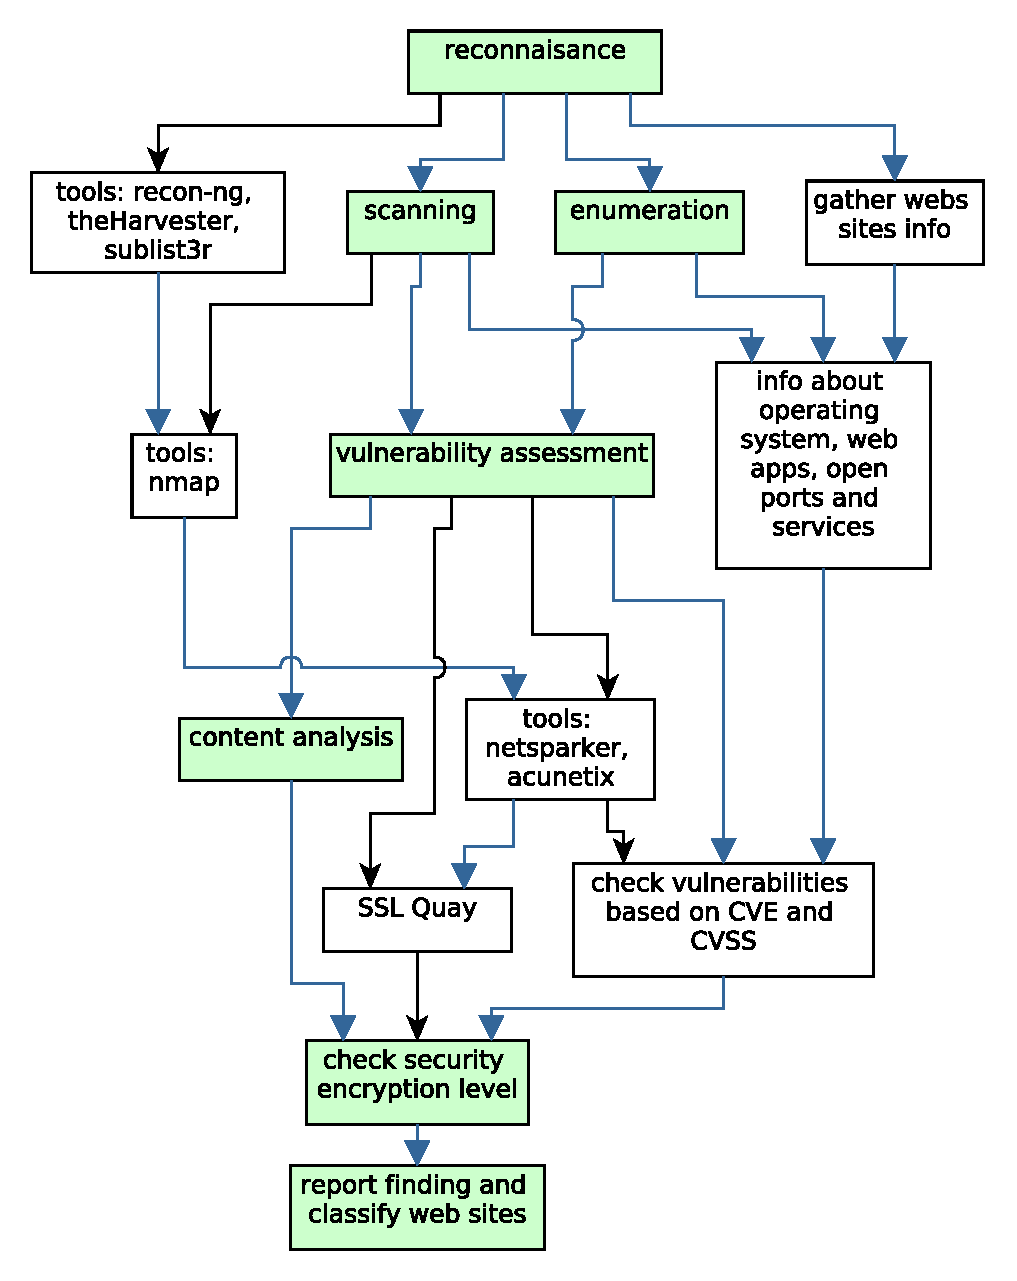
\includegraphics[width=2.5in]{steps.pdf}}
	% where an .eps filename suffix will be assumed under latex, 
	% and a .pdf suffix will be assumed for pdflatex; or what has
	% been declared
	% via \DeclareGraphicsExtensions.
	\caption{Security assessment procedures. This procedures
          consists of four major phases; Reconnaissance, Enumeration
          and Scanning, Vulnerability Assessment, Content
          Analysis. The first three phases are the standard
          procedures. The fourth phase is an additional phase that we
          proposed.}
	\label{fig:steps}
\end{figure}

\subsection{Reconnaissance}

Reconnaissance is the stage when we collect as much as possible
information about the target from Internet, DNS, and, other public
available information.  There are two types of reconnaissance: passive
and active. Passive reconnaissance is to gather information from
search engines and other Internet tools while active reconnaissance is
to gather information from a direct contact with the target through
social engineering.

This study used passive information gathering by searching for all the
Libyan government websites that under the domain \emph{gov.ly}. There
are many open source reconnaissance tools that can be used such as
\emph{recon-ng}, \emph{sublist3r}, \emph{discovery} and,
\emph{theHarvester}\cite{buchanan2017kali}.  In this study,
\emph{TheHarvester} tool have been used to find the sub- domains of
\emph{gov.ly} domain. \emph{TheHarvester} is a tool that uses publicly
available resources from Internet search engines like Google, Bing,
and, Shodan to search for subdomains, hosts, emails and other
information. The command that used in this study was:

\begin{verbatim}
theharvester -d gov.ly -b all > out.txt
\end{verbatim}

The command will save the result in the text file
\verb|out.txt|. 



\subsection{Enumeration}

Enumeration is the phase when we gather information about the network
and information technology infrastructure such as open ports,
operating systems, running services, IPs, status of firewall and,
routers\cite{mehta2018penetration}. There are also two distinct types
of enumeration: active and passive. Passive enumeration is the
utilization of the received packets from a website host and it does
not require any packets to be sent.  Active enumeration is very noisy
which requires packets to be sent and waiting for a reply from the
website host.

When an active enumeration is conducted, the website or the firewall
at the website would detect any attempts from the Internet. Therefore,
any active enumerations are logged by the system, thus would alert the
website owner of a possible cyber attack. For this reason, enumeration
normally done in stealth mode to avoid detection by the websites being
scanned.

This study used active enumeration by using \emph{nmap}\cite{
  lyon2009nmap} to scan for open ports, operating systems, running
services, and main IPs from the Libyan government websites. The
command that has been used in \emph{nmap} scanning is:

\begin{verbatim}
nmap -iL -F -Pn -sV -A -oX
\end{verbatim}

The enumeration phase took a lot of time to be conducted. In this
study, we took two working days to enumerate and to scan all 16
websites using \emph{nmap}. One possible issue was the speed of
network to reach Libyan websites, and another was probably the
websites implemented some security measures to avoid active scanning
and enumeration such as throttling the web traffics.

\subsection{Vulnerability Assessment} 

Vulnerability assessment\cite{shah2015overview} is the phase where we
search for vulnerabilities and flaws in the website’s network
architecture, operating systems, web applications, content management
system and, infrastructures. There are two types of vulnerability
scanning: Manual and Automatic.  Manual vulnerability scanning
requiring advanced skills, experience and may takes a long time. This
normally done by experienced hacker and black
hats\cite{mahmood2010moving}\cite{idris2017vulnerability}.  Automatic
or semi-automatic vulnerability scanning is much faster than
manual. It can be done using open source vulnerabilities scanners like
\emph{Vega} and commercial vulnerabilities scanners like
\emph{Acunetix} or \emph{Netsparker}.  In this study, we used an
automatic method to scan for web applications vulnerabilities using
\emph{Acunetix} and \emph{Netsparker}.



Different web vulnerabilities scanners would produce different results
from one another. This is because each scanner uses different
algorithms to detect and to identify vulnerabilities. For example,
some vulnerabilities are discovered using web vulnerabilities A but
not by web vulnerabilities B, and vice versa. A web vulnerabilities
scanning requires a lot of time because of the software need to crawl
the website and to verify each vulnerability found. A typical web
vulnerability scanning for a typical website will take about 8-15
hour.


In this phase, we also evaluated SSL(Secure Socket Layer) encryption
implementation as part of vulnerability assessment using \emph{Qualys
  SSL}.


\subsubsection{Web Vulnerability Scanning}

In this phase, we used \emph{Acunetix} and \emph{Netsparker} to scan
for web vulnerabilities of the 16 Libyan government websites. The time
required to scan the websites depends on the websites' security,
firewall protections, web application firewall, network speed and
network protection. A typical website scanning takes between 2 and 8
hours. The reports from \emph{Acunetix} are very comprehensive,
depending on the websites complexity. The reports included
vulnerabilities types such as high, medium, low or informational and
their CVE/CVSS rating. The reports doesn't indicate any
counter-measures for the vulnerabilities. A website scanning using
\emph{Netsparker} also takes from 1 to 12 hours. The reports generated
were very extensive and includes CVE/CVSS rating. However,
\emph{Netsparker} reports give some counter-measures for each
vulnerabilities.

This active web vulnerability scan is very noisy and will be logged
into the system log file. The scan could also trigger the firewall or
(Intrusion Detection System) IDS alarm about a possible cyber attack
to the website. Some websites have implemented a counter-measure where
it would block connections from Internet that appears to be an active
scan\cite{stuttard2011web}.

\subsubsection{Secure Socket Layer (SSL) encryption evaluation}


During this phase, we used \emph{Qualys SSL} to evaluate SSL
encryption implementation at each government website. We assume that
it is essential for a government website to implement a secure SSL to
protect the data security on the website. If a government website does
not implement SSL for data transaction, the data will be at risk. Many
government websites deals with highly sensitive and crucial data, and
SSL implementation is an important requirement.

The tool \emph{Qualys SSL} checks for SSL validation, certificate
expiration, cipher strength and, protocol version of SSL
implementation. The results give a detailed and an overall rating for
SSL encryption implementation at the websites. The rating levels are:
\textbf{A}, \textbf{A+} for secure encryption, \textbf{B}, \textbf{C},
\textbf{D}, \textbf{E}, and \textbf{F} means need some updates or
improvements, \textbf{T} is not trusted, usually because of
certificate expiration. If there is no SSL implementation, the
evaluation will indicate as such.  The SSL evaluation takes between 5
to 10 minutes for each website.

\subsection{Content Analysis}

In this phase, we searched for security and privacy policies listed on
the 16 Libyan government websites. The idea is that, if the website is
serious about security and privacy issues, the website will published
the policies on websites for the users. This will indicates that the
websites follow the current standard in security and privacy
issues. This practice also increase the user trust on the
websites. The search was done manually by opening each
website and searched for security and privacy policies links in all
main page sides. We also checked for the availability of the
links provided. Usually, in Arabic websites, security and privacy policies are
named by their Arabic links.

\subsection{Safety level classification}

Based on our experimental previous results, we propose a new safety
classification model based on all three factors: vulnerabilities
analysis, content analysis and SSL encryption assessment. We called
this new classification a website safety level. There are four levels
of safety: highly unsafe(A), somewhat unsafe(B), unsafe(C) and
safe(D).  The basic idea is to combine all security assessment results
and to come up with a safety status by combining all three important
factors as judged by security experts. The safety classification model 
is shown in
Table~\ref{tab:class}.

\begin{table}[thbp]
  \caption{A proposed safety classification model for a website based on
    security assessments, content analysis and SSL encryption
    evaluation. In this model, there are four levels of
    \emph{safe}: A(\emph{highly unsafe}), B(\emph{unsafe}),C(\emph{somewhat unsafe}) and D(\emph{safe}).}
	\label{tab:class}
	\centering
	\begin{tabular}{llclll}
          &  & \multicolumn{4}{c}{\textbf{SSL rating}} \\ \cline{3-6} 
          \textbf{vuln}& \textbf{data} & \textbf{A} & \textbf{B} & \textbf{T} &
                                                                                \textbf{no SSL} \\ \hline
          \multirow{2}{*}{\textit{critical}} & unencrypted & A & A & A & A\\
          & encrypted & B & B & A & A \\ \hline
          \multirow{2}{*}{\textit{high}} & unencrypted & B & B & B & B \\
          & encrypted & C & C & B & B \\ \hline
          \multirow{2}{*}{\textit{medium}} & unencrypted & C & C & B & B \\
          & encrypted & C & C & B & B \\ \hline
          \multirow{2}{*}{\textit{low}} & unencrypted & C & C & B & B \\ &
                                                                           encrypted & D & D & C & B \\ \hline
          \multirow{2}{*}{\textit{info}} & unencrypted & D & D & C & C \\
          \cline{2-6}
          & encrypted & D & D & D & C \\ \hline
	\end{tabular}
	\end{table}


\section{Results and Analysis}


\subsection{Results from Reconnaissance phase}

% In the Reconnaissance phase, we obtained 742 hosts in
% \emph{gov.ly} %domain. We selected 37 websites for further analysis. Lastly,
% we
% only %selected websites which are still relevant and under the current Libyan
% government. After selection, we selected 16 Libyan government websites
% for our study. For anonymity, we have rename each
% website as %$w_1,\ldots,w_{16}$.

We found 742 hosts in the domain and subdomain. The 742 hosts have
been copied into Excel file and classified to get only the main
domains of the government websites. We also check for live websites,
and eliminated dead links and duplicate websites. We identified 37
Libyan government websites under the domain \emph{gov.ly} from our
analysis.

We verified the 37 government websites manually using a web
browser. This verification was important because there were still some
available websites related to the previous government. However, these
websites are not used any more due to Libyan government
transformation.  The verification was conducted by accessing each
website to check for availability of the websites. We also checked
whether the websites were under the control of the current government
``Government of National Accord''. The verification process resulted
in 16 available websites under the current government. The 16
government websites have been changed and indicated by the letter
($w$) followed by a number to protect the confidentiality of the
websites and to avoid abusing the sensitive information that the
experiment might revealed.

\subsection{Results from Enumeration and Scanning phase}


In the Enumeration and Scanning phase, we used \emph{nmap}. From
\emph{nmap}, we discovered the type of operating system used by the
websites, how many open ports were available, the type of running
services and the websites IPs number. The information is summarized in
Table~\ref{tab:nmap}.

\begin{table}[thbp]
  \caption{The results from \emph{nmap} scanning on 16 Libyan
    government websites. We get information about operating system
    (yes/no), the number of open ports(count), type of running
    services(yes/no) and, IP number(yes/no). The websites have been
    changed using name $w_1 \ldots w_{16}$.}
	\label{tab:nmap}
	\centering
	\begin{tabular}{lllll}
          websites & \begin{tabular}[c]{@{}l@{}}operating\\ system\end{tabular} & services & \begin{tabular}[c]{@{}l@{}}open\\ ports\end{tabular} & IP \\ \hline
          $w_1$ & yes & yes & 10 & yes \\
          $w_2$ & no &  no &  2 &  no\\
          $w_3$ & yes & yes & 10 & yes \\
          $w_4$ & yes & yes  & 10  & yes \\
          $w_5$ &  yes & no  & 2   & no \\
          $w_6$ & yes & yes  & 13  & yes \\
          $w_7$ & yes & yes & 11 & yes \\
          $w_8$ & yes & yes & 1 & yes \\
          $w_9$ & yes & yes & 9 & yes \\
          $w_{10}$ & no & yes & 9 & yes  \\
          $w_{11}$ & no & yes & 10 & yes \\
          $w_{12}$ & yes & yes & 11 & yes \\
          $w_{13}$ & yes & yes & 11 & yes \\
          $w_{14}$ & yes & yes & 13 & yes \\
          $w_{15}$ & no & no & 3 & yes \\
          $w_{16}$ & yes & yes & 9 & yes \\ \hline
	\end{tabular}
\end{table}

From the results, we obtained information about operating system from
12 websites. Many of these websites used outdated Window XP and Window Server
or Linux 2.0 series
operating system. The use of outdated operating system could cause a
serious risk for the websites. The operating information could be used
by cyber attackers to launch cyber attacks based on the outdated 
operating system
vulnerabilities. We discovered 13 websites which disclosed their
running services. The information about running services such as \emph{NTP} and 
\emph{telnet} could be used
to launch another type of Internet attacks. We found 11 websites that have
the number of open ports larger than 3. Typically, a website only
needs to open three required ports (HTTP, HTTP, ssh), and close other
ports to reduce attack vectors.

\subsection{Results from Vulnerability Assessment}

In this phase, we used web vulnerabilities scanner \emph{Acunetix} and
\emph{Netsparker}. These two web scanners are the standard tools in
the industry for web scanning. Each tool have its strengths and
drawbacks. The results from the web scanning is shown in
Table~\ref{tab:vuln}.


%	\caption{Results from web vulnerabilities scanning using
% \emph{Acunetix} and \emph{Netsparker}. The are classify into High,
% Medium, Low and Info.}
%\label{tab:vuln}
%\centering



\begin{table}[thbp]
  \caption{Results from web vulnerabilities scanning using
    \emph{Acunetix} and \emph{Netsparker} that indicate the number of
    vulnerabilities for each category High(H), Medium(M), Low(L) and
    Info(I).}
	\label{tab:vuln}
	\centering
	\begin{tabular}{lcllllclll}
          & \multicolumn{4}{c}{Acunetix} &  & \multicolumn{4}{c}{Netsparker} \\ \cline{2-5} \cline{7-10} 
          & H & M & L & I &  & H & M & L & I \\ \cline{2-5} \cline{7-10} 
          $w_1$ & 4 & 17 & 45 & 17 &  & 1 & 2 & 6 & 12 \\
          $w_2$ & 0 & 1 & 0 & 0 &  & 0 & 0 & 4 & 14 \\
          $w_3$ & 0 & 0 & 1 & 1 &  & 1 & 1 & 2 & 7 \\
          $w_4$ & 0 & 1 & 3 & 0 &  & 0 & 0 & 1 & 6 \\
          $w_5$ & 0 & 0 & 0 & 0 &  & 0 & 2 & 1 & 8 \\
          $w_6$ & 0 & 0 & 1 & 0 &  & 1 & 3 & 11 & 24 \\
          $w_7$ & 2 & 91 & 4 & 18 &  & 2 & 2 & 7 & 13 \\
          $w_8$ & 0 & 0 & 1 & 0 &  & 0 & 4 & 3 & 10 \\
          $w_9$ & 0 & 1 & 0 & 0 &  & 0 & 0 & 2 & 5 \\
          $w_{10}$ & 0 & 0 & 1 & 1 &  & 1 & 2 & 10 & 24 \\
          $w_{11}$ & 0 & 0 & 0 & 1 &  & 0 & 1 & 4 & 6 \\
          $w_{12}$ & 0 & 2 & 0 & 1 &  & 0 & 1 & 0 & 9 \\
          $w_{13}$ & 0 & 1 & 1 & 0 &  & 0 & 0 & 1 & 7 \\
          $w_{14}$ & 9 & 1 & 2 & 2 &  & 2 & 3 & 11 & 28 \\
          $w_{15}$ & 0 & 0 & 1 & 0 &  & 0 & 0 & 0 & 8 \\
          $w_{16}$ & 0 & 1 & 2 & 0 &  & 1 & 1 & 4 & 8 \\ \cline{2-5} \cline{7-10} 
          mean &0.94 & 7.25 & 3.86 & 2.56 & & 0.56 & 1.38 & 4.19 & 11.81 \\
          max & 9 & 91 & 45 & 18 & & 2 & 4 & 11 & 28 \\ \hline
	\end{tabular}
\end{table}

From the web vulnerabilities scanning, we obtained 1 critical
vulnerability, 24 high vulnerabilities, 139 medium, 129 low and, 230
informational from 16 websites. We have 1 website with 1 critical 
vulnerability, 7
websites with high vulnerabilities, 15 websites with medium and low
vulnerabilities. Many of the common vulnerabilities are shown in
Table~\ref{tab:common-vulns}.

\begin{table}[thbp]
  \caption{The common vulnerabilities,their risk level and, their
    security impacts.}
	\label{tab:common-vulns}
	\centering
	\begin{tabular}{llll}
          \textbf{vulnerability} & \textbf{count} & \textbf{risk} & \textbf{impact} \\ \hline
          \begin{tabular}[c]{@{}l@{}}application error\\ message\end{tabular} & 78 & medium & \begin{tabular}[c]{@{}l@{}}allow hackers\\ to determine web\\ apps being used\end{tabular} \\ \hline
          \begin{tabular}[c]{@{}l@{}}out of date\\ version of JQuery\end{tabular} & 12 & medium & \begin{tabular}[c]{@{}l@{}}security not \\ patched\end{tabular} \\ \hline
          \begin{tabular}[c]{@{}l@{}}out of date\\ wordpress\end{tabular} & 5 & high & \begin{tabular}[c]{@{}l@{}}security not\\ patches\end{tabular} \\ \hline
          \begin{tabular}[c]{@{}l@{}}cross site\\ scripting\end{tabular} & 5 & high & \begin{tabular}[c]{@{}l@{}}allow hackers to\\ hijack websites\end{tabular} \\ \hline
          CSRF protection & 4 & medium & \begin{tabular}[c]{@{}l@{}}allow hackers to\\ hijack websites\end{tabular} \\ \hline
          PHP disclosure & 3 & medium & \begin{tabular}[c]{@{}l@{}}allow hackers to\\ attack PHP\end{tabular} \\ \hline
          \begin{tabular}[c]{@{}l@{}}PHP DOS\\ vulnerability\end{tabular} & 3 & medium & \begin{tabular}[c]{@{}l@{}}allow hackers to\\ attack PHP\end{tabular} \\ \hline
          out of date PHP & 2 & high & \begin{tabular}[c]{@{}l@{}}security not\\ patches\end{tabular} \\ \hline
          \begin{tabular}[c]{@{}l@{}}data in clear\\ text\end{tabular} & 2 & medium & \begin{tabular}[c]{@{}l@{}}allow hackers to\\ sniff sensitive\\ info\end{tabular} \\ \hline
	\end{tabular}
\end{table} 

The second vulnerability assessment is SSL encryption evaluation. This
step is to determine how a website handle sensitive data such as user
data, login information, privacy and, financial transaction. A secure
website would use an SSL protocol to encrypt data transaction between
the website and the user to ensure the data security. The results is
shown in Table~\ref{tab:ssl}.

%\begin{table}[thbp]
%  \caption{Results from SSL encryption evaluation. The websites were
%	 ranked based on their level of SSL implemenatation. The
%	 ranking are A(secure communication), B{need updates and
%	 improvements}, T(not trusted, certificate expired).}
%	\label{tab:ssl}
%	\begin{tabular}{llllll}
%		& \multicolumn{5}{c}{\textbf{SSL features}} \\ \cline{2-6} 
%                 & \textbf{certificate} & \textbf{\begin{tabular}[c]{@{}l@{}}protocol\\ support\end{tabular}} & \textbf{\begin{tabular}[c]{@{}l@{}}key \\
%           exchange\end{tabular}} & \textbf{\begin{tabular}[c]{@{}l@{}}cipher\\ strength\end{tabular}} & \textbf{\begin{tabular}[c]{@{}l@{}}overall\\
% rating\end{tabular}} \\ \hline
%		$w_1$ & \multicolumn{4}{c}{\textit{no secure protocol}} & \textit{} \\
%		$w_2$ & 100\% & 95\% & 90\% & 90\% & A \\
%		$w_3$ & \multicolumn{4}{c}{\textit{no secure protocol}} & \textit{} \\
%		$w_4$ & 100\% & 95\% & 70\% & 90\% & B \\
%		$w_5$ & 100\% & 95\% & 90\% & 90\% & A \\
%		$w_6$ & 100\% & 95\% & 70\% & 90\% & B \\
%		$w_7$ & \multicolumn{4}{c}{\textit{no secure protocol}} &  \\
%		$w_8$ & - & 90\% & 70\% & 90\% & T \\
%		$w_9$ & 100\% & 95\% & 70\% & 90\% & B \\
%		$w_{10}$ & 100\% & 95\% & 70\% & 90\% & B \\
%		$w_{11}$ & \multicolumn{4}{c}{\textit{no secure protocol}} &  \\
%		$w_{12}$ & 100\% & 95\% & 90\% & 90\% & A \\
%		$w_{13}$ & 100\% & 95\% & 70\% & 90\% & B \\
%		$w_{14}$ & 100\% & 95\% & 70\% & 90\% & B \\
%		$w_{15}$ & 100\% & 95\% & 90\% & 90\% & B \\
%		$w_{16}$ & \multicolumn{4}{c}{\textit{no secure protocol}} &  \\ \hline
%	\end{tabular}
%\end{table}

\begin{table}[thbp]
  \caption{Results from SSL encryption evaluation. The websites were
    ranked based on their level of SSL implementation. The ranking are
    A(secure communication), B{need updates and improvements}, T(not
    trusted, certificate expired) and, no SSL.}
	\label{tab:ssl}
	\centering
	\begin{tabular}{llllll}
          & \multicolumn{5}{c}{\textbf{SSL features}} \\ \cline{2-6} 
          & \textbf{certificate} & \textbf{\begin{tabular}[c]{@{}l@{}}protocol\\ support\end{tabular}} & \textbf{\begin{tabular}[c]{@{}l@{}}key\\ exchange\end{tabular}} & \textbf{\begin{tabular}[c]{@{}l@{}}cipher\\ strength\end{tabular}} & \textbf{\begin{tabular}[c]{@{}l@{}}overall\\ rating\end{tabular}} \\ \hline
          \begin{tabular}[c]{@{}l@{}}$w_1$,$w_7$\\ $w_3$,$w_{11}$\\ $w_{16}$\end{tabular} & \multicolumn{4}{c}{\textit{no secure protocol}} & \textit{} \\ \hline
          \begin{tabular}[c]{@{}l@{}}$w_2$, $w_5$\\ $w_{12}$\end{tabular} & 100\% & 95\% & 90\% & 90\% & A \\ \hline
          \begin{tabular}[c]{@{}l@{}}$w_4$, $w_6$\\ $w_9$, $w_{10}$\\ $w_{13}$,$w_{14}$\\ $w_{15}$\end{tabular} & 100\% & 95\% & 70\% & 90\% & B \\ \hline
          $w_8$ & - & 90\% & 70\% & 90\% & T \\ \hline
	\end{tabular}
\end{table}

In the Content Analysis phase, we manually searched for security and
privacy policies on the 16 websites. Security policy concerns with how
secure is the data being used on the website transaction such as login
information, personal information, financial data and, sensitive
information. Privacy policy concern with whether the website tracks
the users that use the websites by extracting IP number, Geo location,
time of transaction and, personal information. It was to determine
whether the websites informed the users about the security and privacy
policies implemented at the websites.  From our sample 16 websites,
only 3 websites specifically mentioned security and privacy
issues. The others didn't have any links to security or privacy
issues.

\subsection{Safety level classification}

The classification criteria in Table~\ref{tab:class} has been used to
classify the websites into four main safety categories: highly unsafe,
safe, somewhat unsafe, safe. The criteria are based on security
assessment, content analysis and SSL encryption evaluation. Each
website would be manually assessed by a panel of security experts to
determine the safety category of each website. Table~\ref{tab:sum}
showed the safety category and  previous security assessments. The
current approach for safety classification is a heuristic approach. It
is derived based on security assessments and, security experts
experiences.

\begin{table}[thbp]
  \caption{Summary of security assessment, SSL encryption evaluation
    and Content Analysis. For \emph{vulns} column, the number indicate
    the total number of High(H) and Medium(M) vulnerabilities from web
    scanning.Content Analysis column indicate whether the website has
    security policy and has privacy policy(1,1), no security policy
    but has privacy policy(0,1), has security policy but no privacy
    policy(1,0), no security policy and no privacy policy(0,0)
    . Safety category column indicate the safety category: 1(highly
    unsafe), 2(unsafe), 3(somewhat unsafe), 4(safe)}
	\label{tab:sum}
	\centering
	\begin{tabular}{lllll}
          \textbf{website} & \textbf{\begin{tabular}[c]{@{}l@{}} vulns \end{tabular}} & \textbf{SSL} & \textbf{\begin{tabular}[c]{@{}l@{}}Content\\ Analysis\end{tabular}} & \textbf{\begin{tabular}[c]{@{}l@{}}Safety\end{tabular}} \\ \hline
          $w_1$ & 21 & - & (0,0) & 2 \\
          $w_2$ & 1 & A & (1,0) & 3 \\
          $w_3$ & 2 & - & (1,1) & 2 \\
          $w_4$ & 1 & B & (0,0) & 3 \\
          $w_5$ & 2 & A & (0,0) & 3 \\
          $w_6$ & 4 & B & (0,0) & 2 \\
          $w_7$ & 99 & - & (0,0) & 2 \\
          $w_8$ & 4 & T & (0,0) & 3 \\
          $w_9$ & 1 & B & (0,0) & 3 \\
          $w_{10}$ & 3 & B & (0,1) & 2 \\
          $w_{11}$ & 1 & - & (0,0) & 3 \\
          $w_{12}$ & 2 & A & (0,0) & 3 \\
          $w_{13}$ & 1 & B & (0,0) & 3 \\
          $w_{14}$ & 10 & B & (0,0) & 1 \\
          $w_{15}$ & 0 & B & (0,0) & 4 \\
          $w_{16}$ & 2 & - & (0,0) & 2 \\ \hline
	\end{tabular}
\end{table}


\section{Discussion}


Based on the security assessments results, SSL encryption
evaluations and content analysis results, we found that many
Libyan government websites have some vulnerabilities issues and
do not have good security implementations. Enumeration and Scanning
phase has detected a good deal of information about
operating systems, open ports, services, and main IPs about
the websites.  These information might be used by the
attacker to find vulnerabilities of the websites. For
example, some websites wre detected using operating outdated
systems are Windows XP or old versions of Linux (version 2.0
series). These two operating systems have many old
vulnerabilities that could be exploited by hackers.

Open ports are another attack vector for cyber hackers. A
hardened website only needs 3 essential open ports for data
transmission: \emph{HTTP} at port 80, \emph{HTTPS} at port
443 and \emph{SSH} at port 22. All other ports are not
important for a website. Port numbers below 100 are
reserved for system services such as \emph{ftp},
\emph{telnet} and, \emph{NTP}. We found twelve of the 16 websites
have 4 or more open ports and only 4 websites have 3 open
ports or fewer. We opined that if a website have more open ports available, the higher the risk of a cyber attack to a website.
Services from a website are served using open ports. Cyber
hackers can exploit these available services to gain access to the website. Websites should only employed important services
such as \emph{HTTP}, \emph{HTTPS} and, \emph{SSH} only to
reduce the risk of illegal access to a website. Basic services such as
\emph{ftp} and \emph{telnet} could be exploited by cyber
attackers if these services are not properly configured.

Using \emph{Acunetix} and \emph{Netsparker}, we found that 9
of the 16 websites have high or medium vulnerabilities as
shown in Table~\ref{tab:vuln} and, 7 of the 16 websites do
not have high or medium vulnerabilities. That security
implementation at the 16 Libyan government websites are
good but need improvement. There is only 1 website with a
critical vulnerability.

The results from \emph{Acunetix} and \emph{Netsparker} are
different. This is to be expected since both of them use
different algorithms to detect vulnerabilities. Some
vulnerabilities were found by \emph{Acunetix} and not by
\emph{Netsparker} and, vice versa. \emph{Acunetix}
discovered more high and medium vulnerabilities than
\emph{Netsparker}. \emph{Netsparker} discovered more low and
informational vulnerabilities than \emph{Acunetix}.
Therefore, it is good practice to use both web scanners.

The websites with high and medium vulnerabilities might be
compromised or might be open to future cyber attacks.
Therefore, these high and medium vulnerabilities need to be
fixed urgently. Many of these vulnerabilities involve
outdated operating systems and web applications. However,
The websites with low and informational vulnerabilities are
also at risk. Attackers might use this information to find
more critical vulnerabilities, to conduct social engineering
and, to launch phishing attacks. Many of the web
vulnerabilities found at the websites are included in OWASP 2017 top 10 web vulnerabilities: Cross-Site Scripting(XS), Sensitive Data
Exposure (lack of SSL, send sensitive data in clear text),
Using Components with Known Vulnerabilities (outdated
programming language or content management system), Broken
Authentication (expired SSL certificate, outdated SSL)and
Security Configuration (application error logs).

In SSL encryption evaluations, we found only 3 websites with
rating \textbf{A}, which indicate the websites implement the
latest SSL security measures for data security. We found 7
websites rated \textbf{B}, because they have weak SSL
exchange keys. The weak keys would allow attackers to do a
Man-In-The-Middle (MITM) attack and to access the data
communication channel. There are 5 websites with no SSL
implementations. These websites would need to implement SSL
encryption protocol since government websites normally
involves in transferring users credential, private data or
sensitive data through the Internet. We found 1 website with
an expired SSL certificate. Hackers may take advantage of this
website by using MITM attacks or POODLE attacks.

Based our security assessment and content analysis study, we propose
a safe classification model that would categorize the websites into
4 \emph{safe} categories: \emph{highly
	unsafe}, \emph{unsafe}, \emph{somewhat safe}, \emph{safe}.
The criteria are based on the web security assessment, the SSL
encryption evaluation and the content analysis of security and
privacy policies. Based on these criteria, we have 1
\emph{highly unsafe} website because this website involves
in handling Libyan citizen private information and have low
SSL rating. We have 6 \emph{unsafe} websites with a high
number of vulnerabilities and low SSL rating. The websites
need to fix their vulnerabilities and improve their SSL
implementation. We also have 8 \emph{somewhat unsafe}
websites with low numbers of vulnerabilities and low SSL
rating. These websites need to improve their SSL
implementations. We have 1 \emph{safe} website where its has
0 vulnerabilities and low SSL rating. This website might
need some improvement in SSL implementation.  

Based on our proposed \emph{safe} 
classification model, we have 1 \emph{highly 
	unsafe} website, 6 \emph{unsafe} websites, 8 \emph{somewhat
	unsafe} and 1 \emph{safe} website. For a website to have a safe category, we propose for a website to follow these guidelines;
\begin{enumerate}
	\item Eliminate critical and high level vulnerabilities.
	This can be done with regular web vulnerabilities
	assessment. Also, the website needs to update operating
	system regularly, to patch securities holes, to updating
	web apps and, to harden the system.
	\item Implement secure SSL and avoid expired certificate. This will make sure the data communication channel is safe.
	\item Published
	policy on privacy and security. This will install confident for users to use the website for sensitive data transactions.
\end{enumerate} 




  

%\begin{figure}[!t]
%\centering
%\includegraphics[width=2.5in]{myfigure}
% where an .eps filename suffix will be assumed under latex, 
% and a .pdf suffix will be assumed for pdflatex; or what has been declared
% via \DeclareGraphicsExtensions.
%\caption{Simulation results for the network.}
%\label{fig_sim}
%\end{figure}
%
%\begin{figure}
%	\centering
%	\includegraphics[width=2.5in]{Rplot01.pdf}
%	\caption{R plot}
%\end{figure}





\section{Conclusion}

In this paper, we have studied security assessment of 16 Libyan
government websites using a four phases framework: Renaissance,
Enumeration and Scanning, Vulnerability Assessment and Content
Analysis. Our study found 3 websites with more than 9 vulnerabilities and, 12 websites have between 0 and 8 vulnerabilities. Twelve websites implement SSL
encryption at different level of implementation with only 3 websites
have \emph{A} rating. Only 3 websites have published security and
privacy policies on their websites. Based on our \emph{safe} category model, we have 1 \emph{highly unsafe} website due to its SSL implementation and the nature of
its operation. It is highly recommended for the websites to keep
up-to-date with securities issues, system patches and, cyber attacks
vectors. The websites also need to develop security and privacy policies
for their users so the users would trust the websites.

Overall, we considered the Libyan government websites are adequately
secured without major security issues.We encourage the
websites to improve their security implementation by fixing the
vulnerabilities, updating security patches, updating system
configurations and, improving SSL implementations. For future work, this study can be extended to cover all Libyan
government and educational websites. Also, the same study can be
conducted on commercial websites. Then, a comparison can be made
between these websites from a security assessment perspective.




% conference papers do not normally have an appendix


% use section* for acknowledgment
\section*{Acknowledgment}


The authors would like to thank Center for Cybersecurity at Universiti
Kebangsaan Malaysia for their assistance.





% trigger a \newpage just before the given reference
% number - used to balance the columns on the last page
% adjust value as needed - may need to be readjusted if
% the document is modified later
%\IEEEtriggeratref{8}
% The "triggered" command can be changed if desired:
%\IEEEtriggercmd{\enlargethispage{-5in}}

% references section

% can use a bibliography generated by BibTeX as a .bbl file
% BibTeX documentation can be easily obtained at:
% http://mirror.ctan.org/biblio/bibtex/contrib/doc/
% The IEEEtran BibTeX style support page is at:
% http://www.michaelshell.org/tex/ieeetran/bibtex/
%\bibliographystyle{IEEEtran}
% argument is your BibTeX string definitions and bibliography database(s)
%\bibliography{IEEEabrv,../bib/paper}
%
% <OR> manually copy in the resultant .bbl file
% set second argument of \begin to the number of references
% (used to reserve space for the reference number labels box)
%\begin{thebibliography}{1}
%
%\bibitem{IEEEhowto:kopka}
%H.~Kopka and P.~W. Daly, \emph{A Guide to \LaTeX}, 3rd~ed.\hskip 1em plus
%  0.5em minus 0.4em\relax Harlow, England: Addison-Wesley, 1999.
%
%\end{thebibliography}
%\bibliography{crc}
%\bibliographystyle{IEEEtran}

% Generated by IEEEtran.bst, version: 1.14 (2015/08/26)
\begin{thebibliography}{10}
  \providecommand{\url}[1]{#1} \csname url@samestyle\endcsname
  \providecommand{\newblock}{\relax} \providecommand{\bibinfo}[2]{#2}
  \providecommand{\BIBentrySTDinterwordspacing}{\spaceskip=0pt\relax}
  \providecommand{\BIBentryALTinterwordstretchfactor}{4}
  \providecommand{\BIBentryALTinterwordspacing}{\spaceskip=\fontdimen2\font
    plus \BIBentryALTinterwordstretchfactor\fontdimen3\font minus
    \fontdimen4\font\relax} \providecommand{\BIBforeignlanguage}[2]{{%
      \expandafter\ifx\csname l@#1\endcsname\relax \typeout{**
        WARNING: Outran.Best: No hyphenation pattern has been}%
      \typeout{** loaded for the language `#1'. Using the pattern
        for}%
      \typeout{** the default language instead.}%
      \else \language=\csname l@#1\endcsname \fi #2}}
  \providecommand{\BIBdecl}{\relax} \BIBdecl
	
\bibitem{zhao2010opportunities} J.~J. Zhao and S.~Y. Zhao,
  ``Opportunities and threats: A security assessment of state
  e-government websites,'' \emph{Government Information Quarterly},
  vol.~27, no.~1, pp. 49--56, 2010.
	
\bibitem{ismailova2017web} R.~Ismail ova, ``Web site accessibility,
  usability and security: a survey of government web sites in Kirghiz
  republic,'' \emph{Universal Access in the Information Society},
  vol.~16, no.~1, pp. 257--264, 2017.
	
\bibitem{reddick2012channel} C.~G. Red dick and M.~Turner, ``Channel
  choice and public service delivery in Canada: Comparing e-government
  to traditional service delivery,'' \emph{Government Information
    Quarterly}, vol.~29, no.~1, pp. 1--11, 2012.
	
\bibitem{felderer2016security} M.~Felderer, M.~B{\"u}chler, M.~Johns,
  A.~D. Brucker, R.~Breu, and A.~Pretschner, ``Security testing: A
  survey,'' in \emph{Advances in Computers}.\hskip 1em plus 0.5em
  minus 0.4em\relax Elsevier, 2016, vol. 101, pp. 1--51.
	
\bibitem{al2015security} M.~S. Al-Sanea and A.~A. Al-Daraiseh,
  ``Security evaluation of Saudi Arabia's websites using open source
  tools,'' in \emph{2015 First International Conference on
    Anti-Cybercrime (ICACC)}.\hskip 1em plus 0.5em minus 0.4em\relax
  IEEE, 2015, pp. 1--5.
	
\bibitem{yusof2013evaluating} M.~M. Yusof and A.~Y.~A. Yusuff,
  ``Evaluating e-government system effectiveness using an integrated
  socio-technical and fit approach,'' \emph{Information Technology
    Journal}, vol.~12, no.~5, pp. 894--906, 2013.
	
\bibitem{kasimin2013using} H.~Kasimin, A.~Aman, and Z.~M. Noor,
  ``Using evaluation to support organizational learning in
  e-government system: A case of Malaysia government,''
  \emph{International Journal of Electronic Government Research
    (IJEGR)}, vol.~9, no.~1, pp. 45--64, 2013.
	
\bibitem{ahmed2011potential} A.~A. Ahmed, S.~Dalbir, and M.~Ibrahim,
  ``Potential e-commerce adoption strategies for Libyan
  organization,'' \emph{International Journal of Information and
    Communication Technology Research}, 2011.
	
\bibitem{elaswad2016identity} O.~Elaswad and C.~D. Jensen, ``Identity
  management for e-government Libya as a case study,'' in
  \emph{Information Security for South Africa (ISSA), 2016}.\hskip 1em
  plus 0.5em minus 0.4em\relax IEEE, 2016, pp. 106--113.
	
\bibitem{gebba2012government} T.~R. Gebba and M.~R. Zakaria,
  ``E-government in Egypt: An analysis of practices and challenges,''
  \emph{International Journal of Business Research and Development},
  vol.~4, no.~2, 2012.
	
\bibitem{elmansori2017factors} M.~M. Elmansori, H.~Atan, and A.~Ali,
  ``Factors affecting e-government adoption by citizens in Libya: A
  conceptual framework,'' \emph{i-Manager's Journal on Information
    Technology}, vol.~6, no.~4, p.~1, 2017.
	
\bibitem{tehrani2013cyber} P.~M. Tehrani, N.~A. Manap, and H.~Taji,
  ``Cyber terrorism challenges: The need for a global response to a
  multi-jurisdictional crime,'' \emph{Computer Law \& Security
    Review}, vol.~29, no.~3, pp. 207--215, 2013.
	
\bibitem{yusof2011cyber} A.~R.~M. Yusof, M.~F. Sukimi, S.~B. Ismail,
  and Z.~B. Othman, ``The cyber space and information, communication
  and technology: A tool for westernization or orientalism or both,''
  \emph{Journal of Computer Science}, vol.~7, no.~12, pp. 1784--1792,
  2011.
	
\bibitem{ihmouda2013penetration} R.~Ihmouda, N.~H. Alwi~Mohd
  \emph{et~al.}, ``Penetration testing for Libyan government
  website,'' in \emph{International Conference on Computing and
    Informatics}.\hskip 1em plus 0.5em minus 0.4em\relax Universiti
  Utara Malaysia, 2013.
	
\bibitem{forti2017new} Y.~B. Forti and M.~G. Wynn, ``A new model for
  e-government in local level administrations in Libya,'' in \emph{The
    Proceedings of 17th European Conference on Digital Government ECDG
    2017}, 2017, p. 315.
	
\bibitem{IJIR3439} Y.~I. Abuzawayda, ``Security issues on Libya's
  e-government,'' \emph{Imperial Journal of Interdisciplinary
    Research}, vol.~3, no.~1, 2016.
	
\bibitem{awoleye2012technological} O.~M. Awoleye, B.~Ojuloge, and
  W.~O. Siyanbola, ``Technological assessment of e-government web
  presence in Nigeria,'' in \emph{Proceedings of the 6th International
    Conference on Theory and Practice of Electronic Governance}.\hskip
  1em plus 0.5em minus 0.4em\relax ACM, 2012, pp. 236--242.
	
\bibitem{awoleye2014web} O.~M. Awoleye, B.~Ojuloge, and M.~O. Ilori,
  ``Web application vulnerability assessment and policy direction
  towards a secure smart government,'' \emph{Government Information
    Quarterly}, vol.~31, pp. S118--S125, 2014.
	
\bibitem{awang2014survey} N.~F. Awang, A.~A. Manaf, and
  W.~S. Zainudin, ``A survey on conducting vulnerability assessment in
  web-based application,'' in \emph{International Conference on
    Advanced Machine Learning Technologies and Applications}.\hskip
  1em plus 0.5em minus 0.4em\relax Springer, 2014, pp. 459--471.
	
\bibitem{srinivasan2017web} S.~M. Srinivasan and R.~S. Sangwan, ``Web
  app security: A comparison and categorization of testing
  frameworks,'' \emph{IEEE Software}, no.~1, pp.  99--102, 2017.
	
\bibitem{alsmadi2016government} I.~Alsmadi and E.~Abu-Shanab,
  ``E-government website security concerns and citizens' adoption,''
  \emph{Electronic Government, an International Journal}, vol.~12,
  no.~3, pp. 243--255, 2016.
	
\bibitem{antunes2014penetration} N.~Antunes and M.~Vieira,
  ``Penetration testing for web services,'' \emph{Computer}, vol.~47,
  no.~2, pp. 30--36, 2014.
	
\bibitem{mell2006common} P.~Mell, K.~Scarfone, and S.~Romanosky,
  ``Common vulnerability scoring system,'' \emph{IEEE Security \&
    Privacy}, vol.~4, no.~6, 2006.
	
\bibitem{bertino2017botnets} E.~Bertino and N.~Islam, ``Botnets and
  internet of things security,'' \emph{Computer}, no.~2, pp. 76--79,
  2017.
	
\bibitem{owasp10application} T.~F. OWASP, ``Application security
  risks-2017. open web application security project (OWASP),'' 2017.
	
\bibitem{scholte2012have} T.~Scholte, D.~Balzarotti, and E.~Kirda,
  ``Have things changed now? an empirical study on input validation
  vulnerabilities in web applications,'' \emph{Computers \& Security},
  vol.~31, no.~3, pp. 344--356, 2012.
	
\bibitem{munoz2013methods} F.~R. Munoz and L.~G. Villalba, ``Methods
  to test web applications scanners,'' in \emph{Proceedings of the 6th
    International Conference on Information Technology}, 2013.
	
\bibitem{makino2015evaluation} Y.~Makino and V.~Klyuev, ``Evaluation
  of web vulnerability scanners,'' in \emph{Intelligent Data
    Acquisition and Advanced Computing Systems: Technology and
    Applications (IDAACS), 2015 IEEE 8th International Conference on},
  vol.~1.\hskip 1em plus 0.5em minus 0.4em\relax IEEE, 2015,
  pp. 399--402.
	
\bibitem{roldan2017comparison} G.~Rold{\'a}n-Molina, M.~Almache-Cueva,
  C.~Silva-Rabad{\~a}o, I.~Yevseyeva, and V.~Basto-Fernandes, ``A
  comparison of Cybersecurity risk analysis tools,'' \emph{Procedia
    Computer Science}, vol. 121, pp. 568--575, 2017.
	
\bibitem{freier2011secure} A.~Freier, P.~Karlton, and P.~Kocher, ``The
  secure sockets layer (SSL) protocol version 3.0,'' Tech. Rep., 2011.
	
\bibitem{alnatheer2014secure} M.~A. Alnatheer, ``Secure socket layer
  (SSL) impact on web server performance,'' \emph{Journal of Advances
    in Computer Networks}, vol.~2, no.~3, pp. 211--217, 2014.
	
\bibitem{weidman2014penetration} G.~Weidman, \emph{Penetration
    testing: a hands-on introduction to hacking}.\hskip 1em plus 0.5em
  minus 0.4em\relax No Starch Press, 2014.
	
\bibitem{buchanan2017kali} C.~Buchanan and V.~Ramachandran, \emph{Kali
    Linux Wireless Penetration Testing Beginner's Guide: Master
    wireless testing techniques to survey and attack wireless networks
    with Kali Linux, including the CRACK attack}.\hskip 1em plus 0.5em
  minus 0.4em\relax Packt Publishing Ltd, 2017.
	
\bibitem{mehta2018penetration} S.~Mehta, G.~Raj, and D.~Singh,
  ``Penetration testing as a test phase in web service testing a black
  box pen testing approach,'' in \emph{Smart Computing and
    Informatics}.\hskip 1em plus 0.5em minus 0.4em\relax Springer,
  2018, pp.  623--635.
	
\bibitem{lyon2009nmap} G.~F. Lyon, \emph{Nmap network scanning: The
    official Nmap project guide to network discovery and security
    scanning}.\hskip 1em plus 0.5em minus 0.4em\relax Insecure, 2009.
	
\bibitem{shah2015overview} S.~Shah and B.~M. Mehtre, ``An overview of
  vulnerability assessment and penetration testing techniques,''
  \emph{Journal of Computer Virology and Hacking Techniques}, vol.~11,
  no.~1, pp. 27--49, 2015.
	
\bibitem{mahmood2010moving} M.~A. Mahmood, M.~Siponen, D.~Straub,
  H.~R. Rao, and T.~Raghu, ``Moving toward black hat research in
  information systems security: an editorial introduction to the
  special issue,'' \emph{MIS quarterly}, vol.~34, no.~3, pp. 431--433,
  2010.
	
\bibitem{idris2017vulnerability} I.~Idris, M.~U. Majigi,
  S.~Abdulhamid, M.~Olalere, and S.~I. Rambo, ``Vulnerability
  assessment of some key Nigeria government websites,''
  \emph{International Journal of Digital Information and Wireless
    Communications}, vol.~7, no.~3, pp. 143--153, 2017.
	
\bibitem{stuttard2011web} D.~Stuttard and M.~Pinto, \emph{The web
    application hacker's handbook: Finding and exploiting security
    flaws}.\hskip 1em plus 0.5em minus 0.4em\relax John Wiley \& Sons,
  2011.
	
\end{thebibliography}


% that's all folks
\end{document}


